% このディレクトリで2回実行：pdflatex -interaction=nonstopmode -halt-on-error resume4An26w.tex
\documentclass[a4paper,10pt,pdflatex,ja=standard,jafont=ipaex-type1,
  magstyle=real,scale=1]{bxjsarticle}
\usepackage{lmodern}
\usepackage{amsmath,amssymb,mathtools}
\usepackage{geometry}
\geometry{reset,left=22mm,right=22mm,top=20mm,bottom=17mm,
  headheight=13pt,headsep=6mm,footskip=10mm}
\usepackage{xcolor}
\usepackage{enumitem}
\usepackage{array,booktabs,tabularx}
\usepackage{fancyhdr}
\usepackage{lastpage}
\usepackage{tikz}
\usetikzlibrary{arrows.meta}

\definecolor{ink}{HTML}{193A5C}
\definecolor{accent}{HTML}{237D82}
\definecolor{soft}{HTML}{EAF3F3}
\definecolor{muted}{HTML}{52616B}
\newcommand{\coursename}{解析学 II}
\newcommand{\handoutnumber}{4}
\pagestyle{fancy}
\fancyhf{}
\fancyhead[L]{\small\color{ink}\coursename{}・授業要約と演習}
\fancyhead[R]{\small\color{ink}第\handoutnumber 回}
\fancyfoot[C]{\small\color{ink}\thepage/\pageref{LastPage}}
\renewcommand{\headrulewidth}{0.3pt}
\setlength{\parindent}{0pt}
\setlength{\parskip}{2pt}
\setlength{\abovedisplayskip}{5pt}
\setlength{\belowdisplayskip}{5pt}
\setlength{\abovedisplayshortskip}{3pt}
\setlength{\belowdisplayshortskip}{4pt}
\setlist[itemize]{leftmargin=1.8em,itemsep=1pt,topsep=2pt,parsep=0pt}

\newcommand{\handouttitle}[1]{%
  \begin{center}
    {\Large\color{ink}#1}\par\vspace{3mm}
    {\color{accent}\rule{0.88\linewidth}{0.7pt}}
  \end{center}\vspace{-2mm}}
\newcommand{\handout}[2]{%
  \renewcommand{\handoutnumber}{#1}%
  \handouttitle{第#1回\quad #2}}
\newcommand{\topic}[1]{\par\vspace{5pt}%
  {\large\sffamily\mdseries\color{accent}#1}\par\vspace{2pt}}
\newcommand{\keybox}[1]{\par\vspace{3pt}\begingroup
  \setlength{\fboxsep}{4pt}%
  \colorbox{soft}{\parbox{\dimexpr\linewidth-2\fboxsep\relax}{\small #1}}%
  \endgroup\par\vspace{2pt}}
\newenvironment{problems}
  {\begin{enumerate}[leftmargin=2em,itemsep=3pt,topsep=3pt,parsep=0pt,
    font=\color{accent}]}
  {\end{enumerate}}


\newcommand{\examplelabel}[1]{{\sffamily\mdseries\color{ink}#1}}
\newcommand{\problemspace}{\par\vspace{5mm}}
\newcommand{\exercises}{%
  {\color{accent}\hrule height 0.7pt}\vspace{3pt}%
  \topic{演習問題（6題）}%
  {\small 領域と積分範囲を確認し、計算過程も書こう。図を描くと範囲を読み取りやすい。}\par}
\tikzset{
  handout diagram/.style={>={Stealth[length=3.2pt,width=3.2pt]},line join=round,
    every node/.style={font=\scriptsize,text=ink}},
  region/.style={fill=soft,draw=accent,semithick},
  slice/.style={accent,line width=1.8pt},
  guide/.style={muted,densely dashed,thin},
  axis/.style={->,ink,thin}}


% Review Q&A can also be used for actual student feedback when it is available.
\newcommand{\feedback}[2]{%
  \par\addvspace{8pt}\noindent\begin{minipage}{\linewidth}%
  {\color{ink}Q. #1}\par\vspace{2pt}%
  {\color{accent}A. }#2%
  \end{minipage}\par}

\begin{document}
\fontsize{10pt}{13.5pt}\selectfont
\setlength{\abovedisplayskip}{4pt}
\setlength{\belowdisplayskip}{4pt}
% Feedback section: add comments and responses here when available.
\fancyhead[L]{\small\color{ink}\coursename{}・フィードバック}
\handout{4}{前回のコメントへのフィードバック}
% \feedback{comment}{response}
\clearpage

% Previous small-test section: add the questions and solutions here.
\fancyhead[L]{\small\color{ink}\coursename{}・小テスト}
\fancyhead[R]{\small\color{ink}第3回}
\handouttitle{第3回\quad 小テスト}
% Questions and solutions are intentionally blank.
\clearpage

\fancyhead[L]{\small\color{ink}\coursename{}・授業要約と演習}
\fancyhead[R]{\small\color{ink}第\handoutnumber 回}
\handout{4}{重積分の計算と累次積分}\label{lesson-start}
\keybox{到達目標：領域の図から積分範囲を読み取り、累次積分を計算できる。
同じ領域を縦・横の両方に切って表し、計算しやすい順序を選ぼう。}

\topic{長方形上の累次積分}
$a<b$、$c<d$ とし、長方形 $K=[a,b]\times[c,d]$ 上で実数値関数 $f$ が連続とする。
重積分は、1変数の積分を繰り返して計算できる。
$$
 \iint_K f(x,y)\,dx\,dy
 =\int_a^b\left(\int_c^d f(x,y)\,dy\right)dx
 =\int_c^d\left(\int_a^b f(x,y)\,dx\right)dy.
$$
\noindent\begin{minipage}[c]{0.65\linewidth}
内側の積分では、外側の変数を定数として扱う。
右図では $x=x_0$ を固定して $y$ を $c$ から $d$ まで動かし、
その結果を $x$ について積分する。

連続関数 $g,h$ に対し $f(x,y)=g(x)h(y)$ なら
$$
 \iint_K g(x)h(y)\,dx\,dy
 =\left(\int_a^bg(x)\,dx\right)\left(\int_c^dh(y)\,dy\right).
$$
例えば $\displaystyle\iint_{[0,1]^2}xy\,dx\,dy=\frac12\cdot\frac12=\frac14$。
\end{minipage}\hfill
\begin{minipage}[c]{0.32\linewidth}
\centering
\begin{tikzpicture}[handout diagram,x=1cm,y=0.85cm]
 \path[region] (0.6,0.5) rectangle (3.5,2.2);
 \fill[accent!20] (1.9,0.5) rectangle (2.1,2.2);
 \draw[slice,<->] (2,0.55) -- (2,2.15);
 \draw[axis] (0,0) -- (4,0) node[right] {$x$};
 \draw[axis] (0,0) -- (0,2.7) node[above] {$y$};
 \draw[guide] (0,0.5) -- (0.6,0.5);
 \draw[guide] (0,2.2) -- (0.6,2.2);
 \foreach \u/\label in {0.6/a,2/x_0,3.5/b}{
  \draw[guide] (\u,0) -- (\u,0.5);
  \node[below] at (\u,0) {$\label$};}
 \node[left] at (0,0.5) {$c$};
 \node[left] at (0,2.2) {$d$};
 \node at (1.05,1.45) {$K$};
 \node[right] at (2.15,1.4) {先に $dy$};
 \draw[->,accent] (0.7,-0.5) -- (3.4,-0.5)
   node[midway,below] {次に $dx$};
\end{tikzpicture}
\end{minipage}\par

\topic{一般領域：縦に切る・横に切る}
各図では、下の不等式で領域 $D$ を定め、$f$ は $D$ 上で連続とする。
境界関数も対応する閉区間で連続とし、$\phi\le\psi$、$\alpha\le\beta$ とする。
太い線は、外側の変数を固定したときの内側の積分区間を表す。

\noindent\begin{minipage}[t]{0.49\linewidth}
\centering
\examplelabel{縦に切る：$x=x_0$ を固定}

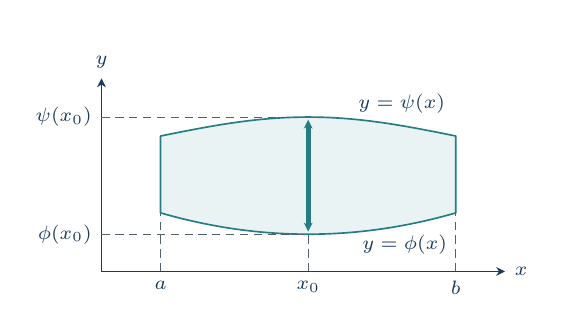
\begin{tikzpicture}[handout diagram,x=1.25cm,y=0.86cm]
 \path[use as bounding box] (-0.75,-0.4) rectangle (4.4,3.6);
 \path[region] plot[domain=0.6:3.6,samples=45]
   (\x,{0.55+0.14*(\x-2.1)^2}) --
   plot[domain=3.6:0.6,samples=45]
   (\x,{2+0.28*sin((\x-0.6)*60)}) -- cycle;
 \draw[axis] (0,0) -- (4.1,0) node[right] {$x$};
 \draw[axis] (0,0) -- (0,2.85) node[above] {$y$};
 \draw[guide] (0,0.55) -- (2.1,0.55);
 \draw[guide] (0,2.28) -- (2.1,2.28);
 \draw[guide] (2.1,0) -- (2.1,0.55);
 \draw[slice,<->] (2.1,0.59) -- (2.1,2.24);
 \node[left] at (0,0.55) {$\phi(x_0)$};
 \node[left] at (0,2.28) {$\psi(x_0)$};
 \node[above] at (3.05,2.19) {$y=\psi(x)$};
 \node[below] at (3.08,0.68) {$y=\phi(x)$};
 \foreach \u/\label in {0.6/a,2.1/x_0,3.6/b}{
  \node[below] at (\u,0) {$\label$};}
 \draw[guide] (0.6,0) -- (0.6,0.865);
 \draw[guide] (3.6,0) -- (3.6,0.865);
\end{tikzpicture}\par
{\small $a\le x\le b,\quad \phi(x)\le y\le\psi(x)$}
$$
 \iint_D f\,dx\,dy
 =\int_a^b\left(\int_{\phi(x)}^{\psi(x)}f\,dy\right)dx.
$$
\end{minipage}\hfill
\begin{minipage}[t]{0.49\linewidth}
\centering
\examplelabel{横に切る：$y=y_0$ を固定}

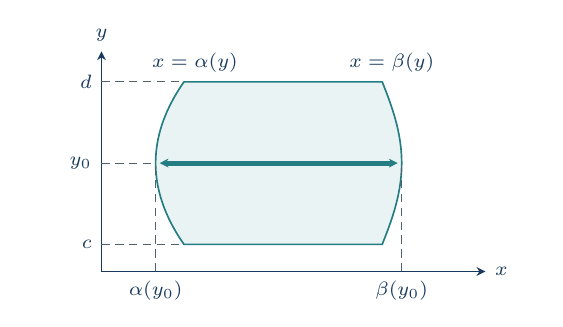
\begin{tikzpicture}[handout diagram,x=1.25cm,y=0.86cm]
 \path[use as bounding box] (-0.75,-0.4) rectangle (4.4,3.6);
 \path[region] plot[domain=0.4:2.8,samples=45]
   ({0.55+0.20*(\x-1.6)^2},\x) --
   plot[domain=2.8:0.4,samples=45]
   ({2.8+0.25*cos((\x-1.6)*65)},\x) -- cycle;
 \draw[axis] (0,0) -- (3.9,0) node[right] {$x$};
 \draw[axis] (0,0) -- (0,3.25) node[above] {$y$};
 \draw[guide] (0,1.6) -- (0.55,1.6);
 \draw[guide] (0.55,0) -- (0.55,1.6);
 \draw[guide] (3.05,0) -- (3.05,1.6);
 \draw[slice,<->] (0.59,1.6) -- (3.01,1.6);
 \node[left] at (0,1.6) {$y_0$};
 \node[below] at (0.55,0) {$\alpha(y_0)$};
 \node[below] at (3.05,0) {$\beta(y_0)$};
 \node[above] at (0.95,2.8) {$x=\alpha(y)$};
 \node[above] at (2.95,2.8) {$x=\beta(y)$};
 \node[left] at (0,0.4) {$c$};
 \node[left] at (0,2.8) {$d$};
 \draw[guide] (0,0.4) -- (0.838,0.4);
 \draw[guide] (0,2.8) -- (0.838,2.8);
\end{tikzpicture}\par
{\small $c\le y\le d,\quad \alpha(y)\le x\le\beta(y)$}
$$
 \iint_D f\,dx\,dy
 =\int_c^d\left(\int_{\alpha(y)}^{\beta(y)}f\,dx\right)dy.
$$
\end{minipage}\par
両方の形で表せるときは、同じ領域を別の不等式で書き直すことで順序を交換できる。

\topic{例：三角形の積分を2通りに計算する}
$D=\{(x,y):0\le y\le x\le1\}$ 上で $f(x,y)=x$ を積分する。
横に切ると、範囲は $0\le y\le1,\ y\le x\le1$ となる。

\noindent\begin{minipage}[c]{0.36\linewidth}
\centering
\begin{tikzpicture}[handout diagram,x=1.4cm,y=1.5cm]
 \path[region] (0,0) -- (1,0) -- (1,1) -- cycle;
 \draw[slice] (0.65,0.02) -- (0.65,0.65);
 \draw[axis] (0,0) -- (1.26,0) node[right] {$x$};
 \draw[axis] (0,0) -- (0,1.22) node[above] {$y$};
 \node[below left] at (0,0) {$0$};
 \node[below] at (1,0) {$1$};
 \node[above left] at (0.57,0.65) {$y=x$};
 \node[below=10pt] at (0.6,0) {先に $dy$};
\end{tikzpicture}\hspace{1mm}
\begin{tikzpicture}[handout diagram,x=1.4cm,y=1.5cm]
 \path[region] (0,0) -- (1,0) -- (1,1) -- cycle;
 \draw[slice] (0.35,0.35) -- (0.98,0.35);
 \draw[guide] (0,0.35) -- (0.35,0.35);
 \draw[axis] (0,0) -- (1.26,0) node[right] {$x$};
 \draw[axis] (0,0) -- (0,1.22) node[above] {$y$};
 \node[below left] at (0,0) {$0$};
 \node[below] at (1,0) {$1$};
 \node[above left] at (0.57,0.65) {$y=x$};
 \node[below=10pt] at (0.6,0) {先に $dx$};
\end{tikzpicture}
\end{minipage}\hfill
\begin{minipage}[c]{0.62\linewidth}
\small
$$
 \begin{aligned}
 \int_0^1\left(\int_0^xx\,dy\right)dx
 &=\int_0^1x^2\,dx=\frac13,\\[6pt]
 \int_0^1\left(\int_y^1x\,dx\right)dy
 &=\frac12\int_0^1(1-y^2)\,dy=\frac13.
 \end{aligned}
$$
\end{minipage}\par
\keybox{内側の積分区間は、切り口の「始点から終点まで」。
順序を変えても領域は同じなので、積分値も一致する。}

\newpage
% Reserve the upper half of page 2 for the remaining summary.
\noindent\begin{minipage}[b][\dimexpr0.5\textheight-\parskip\relax][t]{\linewidth}
\topic{計算しやすい順序を選ぶ}
\noindent\begin{minipage}[c]{0.73\linewidth}
$e^{y^2}$ を $y$ で積分するのは難しいが、$x$ で積分するなら定数として扱える。
領域は $0\le x\le y\le1$。横に切ると $0\le y\le1,\ 0\le x\le y$ となる。
$$
 \begin{aligned}
 \int_0^1\left(\int_x^1 e^{y^2}\,dy\right)dx
 &=\int_0^1\left(\int_0^y e^{y^2}\,dx\right)dy\\
 &=\int_0^1y e^{y^2}\,dy=\frac{e-1}{2}.
 \end{aligned}
$$
最後は $u=y^2$ と置けば、$du=2y\,dy$ を使って計算できる。
\end{minipage}\hfill
\begin{minipage}[c]{0.25\linewidth}
\centering
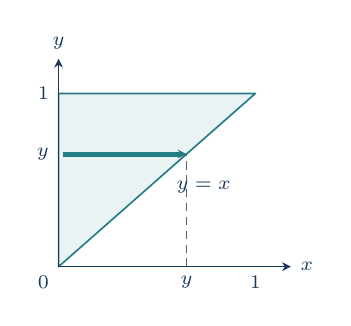
\begin{tikzpicture}[handout diagram,x=2.5cm,y=2.2cm]
 \path[region] (0,0) -- (1,1) -- (0,1) -- cycle;
 \draw[slice,->] (0.02,0.65) -- (0.65,0.65);
 \draw[guide] (0.65,0) -- (0.65,0.65);
 \draw[axis] (0,0) -- (1.18,0) node[right] {$x$};
 \draw[axis] (0,0) -- (0,1.2) node[above] {$y$};
 \node[below left] at (0,0) {$0$};
 \node[below] at (1,0) {$1$};
 \node[left] at (0,1) {$1$};
 \node[left] at (0,0.65) {$y$};
 \node[below] at (0.65,0) {$y$};
 \node[below right] at (0.55,0.55) {$y=x$};
\end{tikzpicture}\par
{\small 横の長さは $y$}
\end{minipage}\par

\topic{対称な領域では、符号の打ち消しを使う}
\noindent\begin{minipage}[c]{0.73\linewidth}
$D$ が $y$ 軸に関して対称で、$f$ は $D$ 上で可積分とする。
さらに $f(-x,y)=-f(x,y)$ なら、左右の点の寄与が打ち消し合い、
$$
 \iint_D f(x,y)\,dx\,dy=0.
$$
例えば円板 $x^2+y^2\le1$ 上の $f(x,y)=xe^{x^2+y^2}$ はこの条件を満たす。
領域と被積分関数の両方を確認しよう。
\end{minipage}\hfill
\begin{minipage}[c]{0.25\linewidth}
\centering
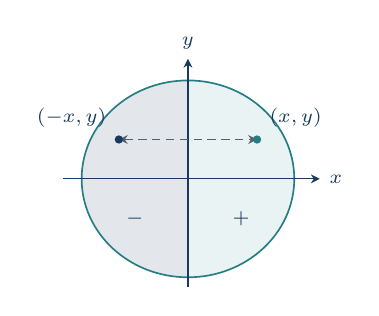
\begin{tikzpicture}[handout diagram,x=1.35cm,y=1.25cm]
 \fill[soft] (0,0) circle (1);
 \fill[ink!12] (0,-1) arc[start angle=270,end angle=90,radius=1] -- cycle;
 \draw[accent,semithick] (0,0) circle (1);
 \draw[axis] (-1.18,0) -- (1.24,0) node[right] {$x$};
 \draw[axis] (0,-1.1) -- (0,1.22) node[above] {$y$};
 \draw[guide,<->] (-0.65,0.4) -- (0.65,0.4);
 \fill[ink] (-0.65,0.4) circle (1.5pt);
 \fill[accent] (0.65,0.4) circle (1.5pt);
 \node[above left=1pt] at (-0.65,0.4) {$(-x,y)$};
 \node[above right=1pt] at (0.65,0.4) {$(x,y)$};
 \node at (-0.5,-0.4) {$-$};
 \node at (0.5,-0.4) {$+$};
\end{tikzpicture}
\end{minipage}\par
\keybox{領域を描く → 外側の変数の範囲を決める → 切り口の両端を読む → 積分する。
切り口の境界が途中で変わるときは、その位置で領域を分けて足し合わせよう。}
{\small\color{muted}補足：ルベーグ積分では、可測集合 $D$ 上の可測関数 $f$ に対し、
$\iint_D|f|<\infty$ ならフビニの定理で順序を交換できる。
$f\ge0$ ならトネリの定理が使え、積分値が $\infty$ でもよい。}\par
\end{minipage}\par\nointerlineskip
% Reserve the lower half of page 2 for exercises and writing space.
\noindent\begin{minipage}[b][0.5\textheight][t]{\linewidth}
\exercises
\begin{problems}
\item \examplelabel{内側の積分。}
$I=\displaystyle\int_0^1\left(\int_0^2(2x+y)\,dy\right)dx$ を求め、積分順序を交換した式も書け。
\problemspace
\item \examplelabel{三角形の領域。}
$D=\{(x,y):0\le y\le x\le1\}$ を描き、$\iint_D(2x+y)\,dx\,dy$ を2通りの積分順序で計算せよ。
\problemspace
\item \examplelabel{曲線に囲まれた領域。}
$D=\{(x,y):0\le x\le1,\ x^2\le y\le x\}$ を描き、横に切ったときの積分範囲を示せ。また、$\iint_Dxy\,dx\,dy$ を求めよ。
\problemspace
\item \examplelabel{計算しやすい順序。}
$I=\displaystyle\int_0^1\left(\int_{\sqrt y}^1e^{x^3}\,dx\right)dy$ の領域を描き、積分順序を変えて計算せよ。
\problemspace
\item \examplelabel{直線で囲まれた領域。}
$D=\{(x,y):x\ge0,\ y\ge0,\ x+y\le1\}$ 上の $\iint_D(1+x)\,dx\,dy$ を求めよ。
\problemspace
\item \examplelabel{対称性で消える項。}
$D=[-1,1]\times[-1,1]$ 上の $I=\iint_D\bigl(xe^{x^2+y^2}+y^2\bigr)\,dx\,dy$ を、対称性を利用して求めよ。
\problemspace
\end{problems}
\end{minipage}

\newpage
\handouttitle{第4回\quad 演習問題の解答}
{\small 各問の被積分関数は対応する有界な閉領域上で連続なので、積分順序を交換できる。}\par
\begin{problems}
\setlength{\itemsep}{5pt}
\item \examplelabel{内側の積分。}
内側では $x$ を定数として扱う。逆順では $y$ を定数として扱うので、
$$
 \begin{aligned}
 \int_0^2(2x+y)\,dy
 &=\left[2xy+\frac{y^2}{2}\right]_{y=0}^{y=2}=4x+2,\\
 I&=\int_0^1(4x+2)\,dx=\left[2x^2+2x\right]_0^1=4,\\
 I&=\int_0^2\left(\int_0^1(2x+y)\,dx\right)dy
 =\int_0^2(1+y)\,dy=4.
 \end{aligned}
$$

\item \examplelabel{三角形の領域。}
$D$ の頂点は $(0,0),(1,0),(1,1)$。
縦に切ると $0\le x\le1,\ 0\le y\le x$、
横に切ると $0\le y\le1,\ y\le x\le1$ である。
$$
 \begin{aligned}
 \iint_D(2x+y)\,dx\,dy
 &=\int_0^1\left(\int_0^x(2x+y)\,dy\right)dx
 =\int_0^1\frac52x^2\,dx=\frac56,\\
 &=\int_0^1\left(\int_y^1(2x+y)\,dx\right)dy
 =\int_0^1(1+y-2y^2)\,dy=\frac56.
 \end{aligned}
$$

\item \examplelabel{曲線に囲まれた領域。}
$x^2=x$ より交点は $(0,0),(1,1)$。この間で $x^2\le x$ となる。
\par\noindent\begin{minipage}[c]{0.72\linewidth}
横に切ると、$x\ge0$ と $x^2\le y\le x$ より
$0\le y\le1,\ y\le x\le\sqrt y$ である。
$$
 \begin{aligned}
 \iint_Dxy\,dx\,dy
 &=\int_0^1\left(\int_{x^2}^xxy\,dy\right)dx\\
 &=\frac12\int_0^1(x^3-x^5)\,dx
 =\frac12\left(\frac14-\frac16\right)=\frac1{24}.
 \end{aligned}
$$
\end{minipage}\hfill
\begin{minipage}[c]{0.26\linewidth}
\centering
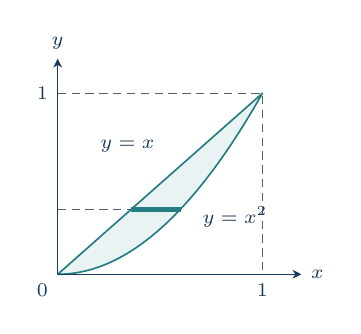
\begin{tikzpicture}[handout diagram,x=2.6cm,y=2.3cm]
 \path[region] plot[domain=0:1,samples=45] (\x,{\x*\x}) -- cycle;
 \draw[slice] (0.36,0.36) -- (0.6,0.36);
 \draw[guide] (0,0.36) -- (0.36,0.36);
 \draw[axis] (0,0) -- (1.19,0) node[right] {$x$};
 \draw[axis] (0,0) -- (0,1.19) node[above] {$y$};
 \node[below left] at (0,0) {$0$};
 \node[below] at (1,0) {$1$};
 \node[left] at (0,1) {$1$};
 \draw[guide] (0,1) -- (1,1) -- (1,0);
 \node[above left] at (0.52,0.62) {$y=x$};
 \node[below right] at (0.66,0.43) {$y=x^2$};
\end{tikzpicture}
\end{minipage}\par

\item \examplelabel{計算しやすい順序。}
$0\le y\le1,\ \sqrt y\le x\le1$ は
$0\le x\le1,\ 0\le y\le x^2$ と同じ領域で、放物線の下側である。
内側では $e^{x^3}$ が定数となり、積分区間の長さは $x^2$ なので、
$$
 I=\int_0^1\left(\int_0^{x^2}e^{x^3}\,dy\right)dx
 =\int_0^1x^2e^{x^3}\,dx
 =\frac13\int_0^1e^u\,du=\frac{e-1}{3}.
$$
ここで $u=x^3$、$du=3x^2\,dx$ と置いた。

\item \examplelabel{直線で囲まれた領域。}
頂点は $(0,0),(1,0),(0,1)$ で、$0\le x\le1,\ 0\le y\le1-x$ と表せる。
$$
 \begin{aligned}
 \iint_D(1+x)\,dx\,dy
 &=\int_0^1\left(\int_0^{1-x}(1+x)\,dy\right)dx\\
 &=\int_0^1(1+x)(1-x)\,dx
 =\left[x-\frac{x^3}{3}\right]_0^1=\frac23.
 \end{aligned}
$$

\item \examplelabel{対称性で消える項。}
$y$ を固定すると、$(-x)e^{(-x)^2+y^2}=-xe^{x^2+y^2}$。
$x$ の積分区間は $[-1,1]$ なので奇関数の積分は0となる。
$$
 \int_{-1}^1xe^{x^2+y^2}\,dx=0,\qquad
 I=\int_{-1}^1\left(\int_{-1}^1y^2\,dx\right)dy
 =2\left[\frac{y^3}{3}\right]_{-1}^1=\frac43.
$$
\end{problems}
\end{document}
